% !TEX TS-program = pdflatex
% !TEX encoding = UTF-8 Unicode

% This is a simple template for a LaTeX document using the "article" class.
% See "book", "report", "letter" for other types of document.

\documentclass[11pt]{article} % use larger type; default would be 10pt

\usepackage[utf8]{inputenc} % set input encoding (not needed with XeLaTeX)

%%% Examples of Article customizations
% These packages are optional, depending whether you want the features they provide.
% See the LaTeX Companion or other references for full information.

%%% PAGE DIMENSIONS
\usepackage{geometry} % to change the page dimensions
\geometry{a4paper} % or letterpaper (US) or a5paper or....
% \geometry{margin=2in} % for example, change the margins to 2 inches all round
% \geometry{landscape} % set up the page for landscape
%   read geometry.pdf for detailed page layout information

\usepackage{graphicx} % support the \includegraphics command and options

% \usepackage[parfill]{parskip} % Activate to begin paragraphs with an empty line rather than an indent

%%% PACKAGES
\usepackage{booktabs} % for much better looking tables
\usepackage{array} % for better arrays (eg matrices) in maths
%\usepackage{paralist} % very flexible & customisable lists (eg. enumerate/itemize, etc.)
\usepackage{verbatim} % adds environment for commenting out blocks of text & for better verbatim
\usepackage{subfig} % make it possible to include more than one captioned figure/table in a single float
% These packages are all incorporated in the memoir class to one degree or another...

%%% HEADERS & FOOTERS
\usepackage{fancyhdr} % This should be set AFTER setting up the page geometry
\pagestyle{fancy} % options: empty , plain , fancy
\renewcommand{\headrulewidth}{0pt} % customise the layout...
\lhead{}\chead{}\rhead{}
\lfoot{}\cfoot{\thepage}\rfoot{}

%%% SECTION TITLE APPEARANCE
\usepackage{sectsty}
\allsectionsfont{\sffamily\mdseries\upshape} % (See the fntguide.pdf for font help)
% (This matches ConTeXt defaults)

%%% ToC (table of contents) APPEARANCE
\usepackage[nottoc,notlof,notlot]{tocbibind} % Put the bibliography in the ToC
\usepackage[titles,subfigure]{tocloft} % Alter the style of the Table of Contents
\renewcommand{\cftsecfont}{\rmfamily\mdseries\upshape}
\renewcommand{\cftsecpagefont}{\rmfamily\mdseries\upshape} % No bold!

%%% END Article customizations

\usepackage[spanish]{babel}
\usepackage{listings} 
%%% The "real" document content comes below...

\title{Investigación de Lenguajes - Pascal}
\author{Rodrigo Castro}
%\date{} % Activate to display a given date or no date (if empty),
         % otherwise the current date is printed 

\begin{document}
\maketitle
%\tableofcontents % No hace falta un TOC en un artículo corto

\section{Introducción}



\section{Características}

\section{Historia}


\section{Tutorial de Instalación}
Un interprete que podemos utilizar para programar en Lisp es DrRacket. Su instalacion es muy sencilla y rapida.
El entorno de trabajo para programar en este lenguaje se puede apreciar en la Figura 5

\begin{figure}[h]
\centering
    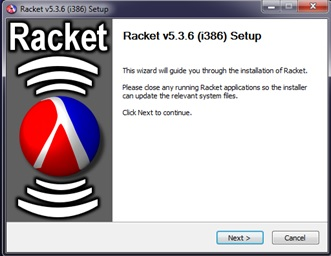
\includegraphics{imagenes_investigacion/paso_uno.jpg}
\caption {}
\label{Figura 1}
\end{figure}

\begin{figure}[h]
\centering
    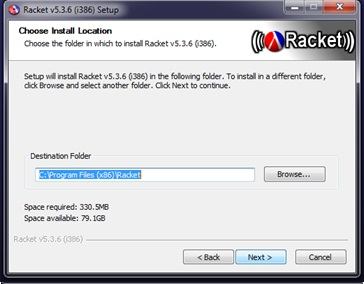
\includegraphics{imagenes_investigacion/paso_dos.jpg}
\caption { }
\label{Figura 2}
\end{figure}

\begin{figure}[h]
\centering
    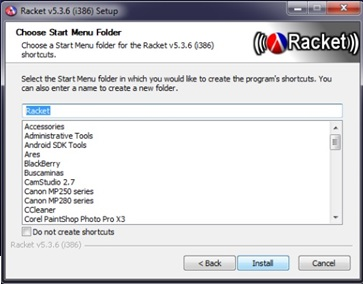
\includegraphics{imagenes_investigacion/paso_tres.jpg}
\caption { }
\label{Figura 3}
\end{figure}

\begin{figure}[h]
\centering
    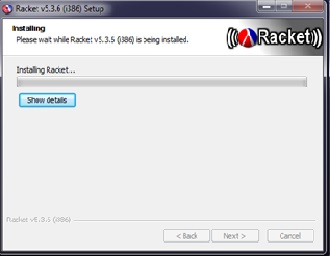
\includegraphics{imagenes_investigacion/paso_cuatro.jpg}
\caption { }
\label{Figura 4}
\end{figure}


\begin{figure}[h]
\centering
    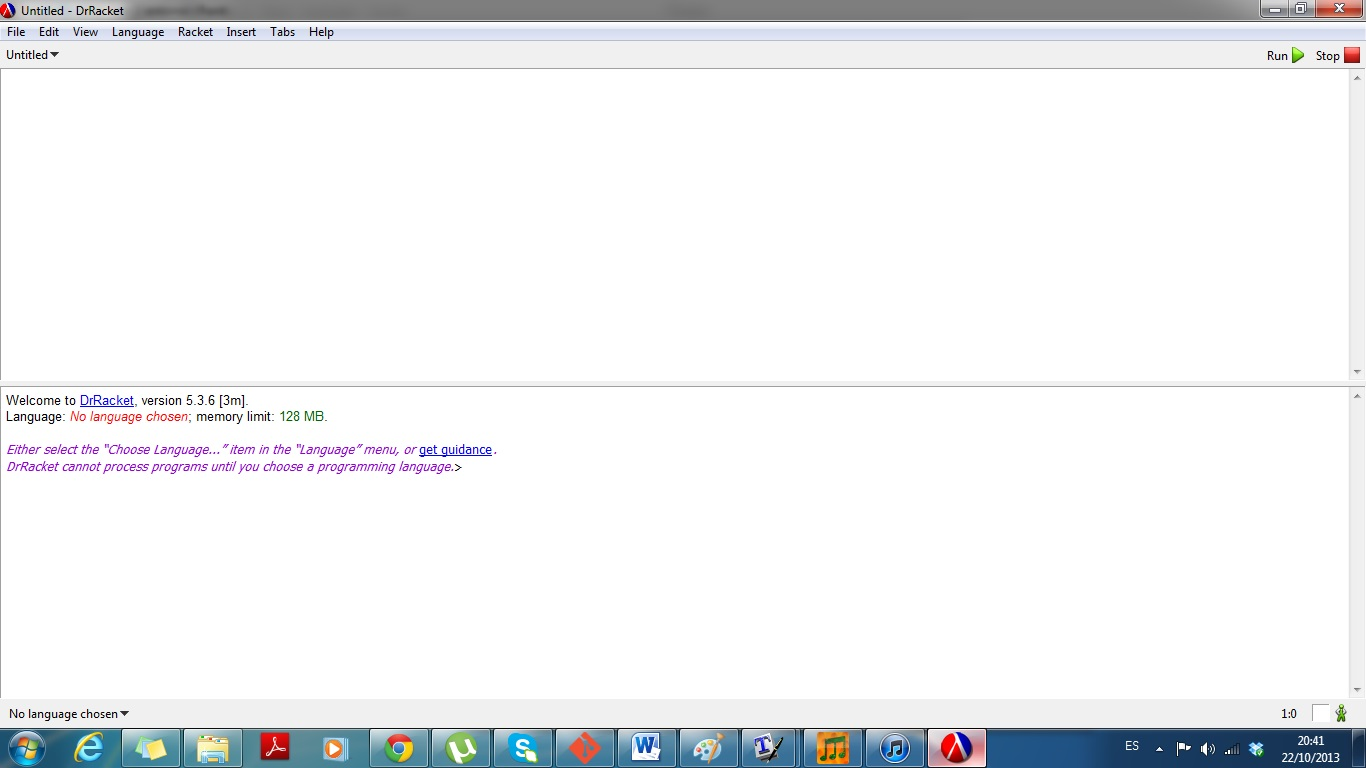
\includegraphics[width=450pts] {imagenes_investigacion/entorno.jpg}
\caption {//Entorno de trabajo de DrRocket}
\label{Figura 5}
\end{figure}


%\section{Hola Mundo y otros Programas Introductorios}


%\lstset{language=Pascal}          % Set your language (you can change the language for each code-block optionally)

%\begin{lstlisting}[frame=single]  % Start your code-block
%for i:=maxint to 0 do
%begin
%{ do nothing }
%end;
%Write('Case insensitive ');
%Write('Pascal keywords.');
%\end{lstlisting}



\end{document}